\chapter{PROJECT GENERAL FRAMEWORK}

\section{Introduction}
\label{sec:introduction}

This chapter provides an overview of the context surrounding our graduation project, beginning with a presentation of the host organization, E-TAFAKNA, where we developed our solution. We will analyze the specific issues that motivated this initiative, then explain the original idea we proposed. Finally, we will summarize the detailed procedures we followed to ensure the smooth progress and successful completion of the project.

\section{Host Organization Presentation}
\label{sec:host-organization}

Founded in 2022, E-Tafakna stands as a trailblazing Tunisian LegalTech startup transforming legal document management across the \ac{MENA} region \cite{wearetech2024etafakna}. Through its intuitive web and mobile platform, the company enables users to seamlessly create, collaborate on, sign, and monitor legal documents from any location, effectively digitizing the entire contract lifecycle.

\begin{figure}[H]
\centering

\includegraphics[width=0.18\textwidth]{figures/logo_E-tafakna.png}
\caption{E-Tafakna Company Logo \cite{etafakna2024website}}
\label{fig:logo-etafakna}
\end{figure}

E-Tafakna distinguishes itself through a deeply user-centric philosophy. The platform offers over 100 pre-designed contract templates covering everything from non-disclosure agreements to employment contracts, coupled with real-time document status tracking and trilingual support in Arabic, French, and English. This strategic combination of simplicity and robust functionality democratizes access to professional legal services, making them affordable and accessible for freelancers, entrepreneurs, and \ac{SME}s. Recognized with the prestigious StartUp'Act label and winner of the HiiL Innovating Justice Challenge 2024, E-Tafakna continues to solidify its position as a regional leader in legal innovation \cite{wearetech2024etafakna}.

\needspace{6\baselineskip}
\section{General Project Overview}
\label{sec:general-overview}

\subsection{Project Framework}

Legal services have long been associated with complexity, high costs, and limited accessibility, 
particularly for individuals, freelancers, and small businesses navigating an increasingly 
regulated environment. The digitalization of these services has become a strategic priority, 
as modern users expect instant, accurate, and accessible legal support. In this context, 
\ac{AI} is emerging as a transformative force, enabling platforms to automate complex legal 
tasks, centralize expertise, and deliver seamless experiences across multiple channels.

E-Tafakna addresses this need through a comprehensive legal platform that covers the entire 
contract lifecycle. Its services span contract template creation, professional consulting, 
document management, real-time contract collaboration, and electronic signature. To further 
enhance this offering, E-Tafakna has integrated two intelligent \ac{AI} agents: Elyssa, a 
smart legal co-pilot focused on document drafting and compliance, and Kahina, an intelligent 
legal avatar designed to explain laws, contracts, and regulations through natural conversation. 
Together, these agents position E-Tafakna as a pioneer in \ac{AI}-powered LegalTech across 
the \ac{MENA} region.

\subsection{Study of Existing Solutions}

E-Tafakna currently offers two \ac{AI}-powered agents to assist users with their legal needs.

\textbf{Elyssa} is a smart legal co-pilot designed to assist users throughout the document 
drafting and review process. It provides:

\begin{itemize}
    \item \textbf{Legal Chatbot:} Instant legal assistance through a conversational interface.
    \item \textbf{Clause Assistant:} Smart generation of contract clauses tailored to the 
    user's context.
    \item \textbf{Contract Analyzer:} Automatic identification of risks and missing clauses 
    within uploaded documents.
    \item \textbf{Compliance Scorer:} Rates contracts against legal standards and suggests 
    targeted improvements.
\end{itemize}

\textbf{Kahina} is an intelligent legal avatar built to make legal knowledge accessible to 
\ac{SME}s, freelancers, and startups. It provides:

\begin{itemize}
    \item \textbf{Legal Intelligence:} Helps users understand legal concepts, procedures, 
    and applicable regulations.
    \item \textbf{Virtual Assistant:} Delivers contextual guidance tailored to the user's 
    specific questions.
    \item \textbf{Multilingual Support:} Communicates fluently in Arabic, French, and English.
    \item \textbf{Conversational Avatar:} Simulates human-like legal consultations for a 
    more natural user experience.
\end{itemize}

Together, Elyssa and Kahina form the intelligent core of E-Tafakna's platform, each serving 
a distinct but complementary role: Elyssa focuses on document-level assistance, while Kahina 
handles broader legal understanding and user guidance \cite{etafakna2024website}.

\subsection{Critical Analysis of the Existing System}

While Elyssa and Kahina represent meaningful advances in accessible legal assistance, 
a critical analysis reveals that the current system still falls short of its full potential. 
Kahina's conversational avatar interface has already addressed the interaction barriers 
previously faced by users, offering multilingual dialogue in Arabic, French, and English. 
However, two fundamental limitations remain unresolved:

\begin{itemize}
    \item \textbf{Lack of Tunisian Legal Specificity:} Both Elyssa and Kahina rely on 
    general-purpose language models that were not trained on Tunisian legal texts. As a 
    result, responses often lack the precision required for local legal matters, missing 
    the nuances of Tunisian legislation, procedures, and regulatory frameworks.

    \item \textbf{Dependency on External Cloud Services:} The current \ac{AI} 
    infrastructure relies on external cloud-based \ac{API}s, which raises concerns around 
    data sovereignty, response latency, and compliance with Tunisian data regulations. 
    E-Tafakna's planned deployment at \ac{ATI} Tunisie requires a fully on-premises 
    solution with no external dependencies, ensuring that all legal data remains within 
    a secure and controlled local infrastructure, which is a requirement the current system
    cannot fulfill.
\end{itemize}

These two limitations, namely insufficient Tunisian legal knowledge and reliance on external
cloud services, define the core technical challenge that our project aims to address.

\subsection{Problem Statement}

The analysis of E-Tafakna's existing \ac{AI} agents reveals a clear and twofold 
challenge. First, both Elyssa and Kahina operate on general-purpose language models 
that lack the domain-specific knowledge required to handle Tunisian legal content 
with the accuracy and reliability that legal matters demand. Second, the current 
architecture depends on external cloud services, making it incompatible with the 
on-premises deployment requirements of \ac{ATI} Tunisie, where data sovereignty 
and infrastructure autonomy are non-negotiable constraints.

This raises a central research question: \textit{How can we build a legal \ac{AI} 
assistant that is both deeply grounded in Tunisian law and fully deployable within 
a secure, self-contained local infrastructure?}

Addressing this question requires tackling three concrete technical problems:

\begin{itemize}
    \item \textbf{Domain Adaptation:} General-purpose language models must be 
    specialized through fine-tuning on a curated corpus of Tunisian legal texts, 
    enabling them to understand the specific terminology, structure, and logic of 
    local legislation.

    \item \textbf{Knowledge Retrieval:} Fine-tuning alone is insufficient for 
    handling the breadth and evolving nature of legal knowledge. A \ac{RAG} pipeline 
    must be designed to allow the model to dynamically retrieve relevant legal 
    documents at inference time, improving both accuracy and up-to-date coverage.

    \item \textbf{Local Deployment:} The resulting system must be optimized to run 
    efficiently on on-premises infrastructure at \ac{ATI} Tunisie, without relying 
    on any external \ac{API} or cloud service, ensuring full data sovereignty and 
    regulatory compliance.
\end{itemize}

\subsection{Proposed Solution}

To address the identified challenges, we propose the development of a domain-specific 
legal \ac{AI} assistant built around two complementary components: a fine-tuned 
\ac{SLM} or \ac{LLM} specialized in Tunisian law, and a \ac{RAG} pipeline designed 
to dynamically incorporate legal knowledge at inference time. The resulting system 
will be deployed entirely on-premises at \ac{ATI} Tunisie, with no dependency on 
external cloud services.

\subsubsection*{Component 1: Fine-Tuned Language Model}

Rather than relying on a generic pre-trained model, we will fine-tune a base 
\ac{SLM} or \ac{LLM} on a curated corpus of Tunisian legal documents, including 
legislation, regulatory texts, and legal procedures. This supervised fine-tuning 
process will enable the model to internalize the specific vocabulary, structure, 
and reasoning patterns of Tunisian law, producing responses that are more accurate, 
contextually appropriate, and legally sound than those of a general-purpose model.

\subsubsection*{Component 2: Retrieval-Augmented Generation Pipeline}

Fine-tuning alone cannot capture the full breadth of Tunisian legal knowledge, nor 
can it account for legislative updates over time. To overcome this, we will design 
a \ac{RAG} pipeline that connects the language model to a vector database populated 
with indexed legal documents. At inference time, the system will retrieve the most 
relevant legal excerpts based on the user's query and inject them into the model's 
context, significantly improving the precision and coverage of generated responses.

\subsubsection*{Component 3: On-Premises Deployment at ATI Tunisie}

The complete system, including the language model, \ac{RAG} pipeline, and vector database, will
be deployed locally on \ac{ATI} Tunisie's infrastructure using Ollama as the local 
\ac{LLM} inference framework. This architecture guarantees full data sovereignty, 
eliminates latency caused by external \ac{API} calls, and ensures compliance with 
Tunisian data regulations. All legal data processed by the system remains within 
ATI's secure on-premises environment.

\subsubsection*{Expected Outcomes}

This solution is expected to deliver the following improvements over the existing system:

\begin{itemize}
    \item \textbf{Higher Legal Accuracy:} Domain-specific fine-tuning ensures the 
    model understands and correctly applies Tunisian legal concepts, reducing 
    erroneous or imprecise responses.

    \item \textbf{Up-to-Date Legal Knowledge:} The \ac{RAG} pipeline allows the 
    system to retrieve current legal documents dynamically, keeping responses 
    relevant even as legislation evolves.

    \item \textbf{Full Data Sovereignty:} On-premises deployment at \ac{ATI} Tunisie 
    ensures that no legal data leaves the organization's infrastructure, meeting 
    both internal security requirements and national data regulations.

    \item \textbf{Seamless Integration:} The system is designed to integrate with 
    E-Tafakna's existing platform, enhancing the capabilities of both Elyssa and 
    Kahina without requiring changes to the user-facing interface.
\end{itemize}

Together, these components form a cohesive and technically grounded solution that 
directly addresses each of the three problems identified in the problem statement, 
transforming E-Tafakna's legal \ac{AI} offering into a specialized, autonomous, 
and locally sovereign system.

\section{Adopted Methodology}
\label{sec:methodology}

Choosing the right methodology is one of the most consequential decisions in any 
technical project. It determines not only how the work is organized, but how 
decisions are made, how progress is measured, and how results are ultimately 
validated. In the context of an \ac{AI}-driven system designed for a real-world 
legal environment, this choice carries particular weight.

\subsection{Methodological Framework Selection}

A wide range of methodological frameworks exists for guiding the development of 
software and intelligent systems. These can be broadly grouped into two families: 
traditional project management methodologies, and data science or research-oriented 
methodologies.

\textbf{Traditional project management methodologies}, such as Scrum and Kanban, 
are general-purpose frameworks focused on how a team organizes and delivers work. 
Scrum structures development into fixed-length iterations called sprints, with 
regular reviews and adaptation cycles, while Kanban emphasizes continuous flow and 
visual task management. Both are well-suited for software delivery projects where 
requirements are relatively stable and the primary challenge is coordination and 
delivery pace. However, they do not address the specific challenges inherent to 
\ac{AI} development, they provide no guidance on data collection, model training, 
evaluation of predictive performance, or the construction and validation of a 
research artifact. Applying them alone to a project involving fine-tuning a language 
model and building a \ac{RAG} pipeline would leave the most critical technical and 
scientific dimensions of the work entirely unguided.

\textbf{Data science and research-oriented methodologies}, by contrast, are designed 
precisely for projects where the core challenge is building, evaluating, and 
deploying an intelligent system or a research artifact. In the field of data science 
and intelligent systems design, several such frameworks have been proposed. These 
range from traditional process-oriented approaches, such as \ac{CRISP-DM} 
\cite{chapman2000crispdm} and \ac{TDSP} \cite{microsoft2016tdsp}, to 
research-centered paradigms such as \ac{DSR} \cite{hevner2004design, peffers2007dsrm}. 
Each addresses a different type of project and carries distinct strengths and 
limitations that must be carefully weighed against the specific requirements at hand.

Our project presents a specific set of requirements that constrain this choice:

\begin{itemize}
    \item \textbf{Domain Specialization:} Fine-tuning a language model on Tunisian 
    legal texts requires multiple cycles of data preparation, training, and evaluation 
    before acceptable performance is achieved.
    \item \textbf{Pipeline Complexity:} Integrating a fine-tuned model with a \ac{RAG} 
    pipeline and a vector database introduces interdependencies between components that 
    must be developed, tested, and refined in coordination.
    \item \textbf{Deployment Constraints:} The on-premises deployment at \ac{ATI} 
    Tunisie imposes strict infrastructure requirements that must be addressed from the 
    earliest stages of the project.
    \item \textbf{Artifact-Centered Development:} The primary deliverable of this 
    project is a concrete technological artifact, a specialized legal chatbot, whose 
    utility must be rigorously designed, built, and evaluated within an academic 
    framework.
\end{itemize}

The following sections present an overview of each candidate methodology and the 
rationale behind our final selection.

\subsection{Overview of CRISP-DM}

\ac{CRISP-DM} \cite{chapman2000crispdm} is a traditional process model that emerged 
in the late 1990s to standardize the practice of data mining, the automated 
extraction of patterns and knowledge from large datasets. It was conceived as an 
industry-neutral framework applicable across sectors and tools, structured around 
six sequential phases \cite{chapman2000crispdm}:

\begin{itemize}
    \item \textbf{Business Understanding:} Defining project objectives and requirements 
    from a business perspective.
    \item \textbf{Data Understanding:} Collecting initial data and identifying quality 
    issues and relevant subsets.
    \item \textbf{Data Preparation:} Cleaning, transforming, and structuring data for 
    modeling.
    \item \textbf{Modeling:} Applying modeling techniques and calibrating parameters 
    for optimal results.
    \item \textbf{Evaluation:} Assessing the model against business objectives.
    \item \textbf{Deployment:} Integrating the model into operational systems.
\end{itemize}

\begin{figure}[H]
\centering
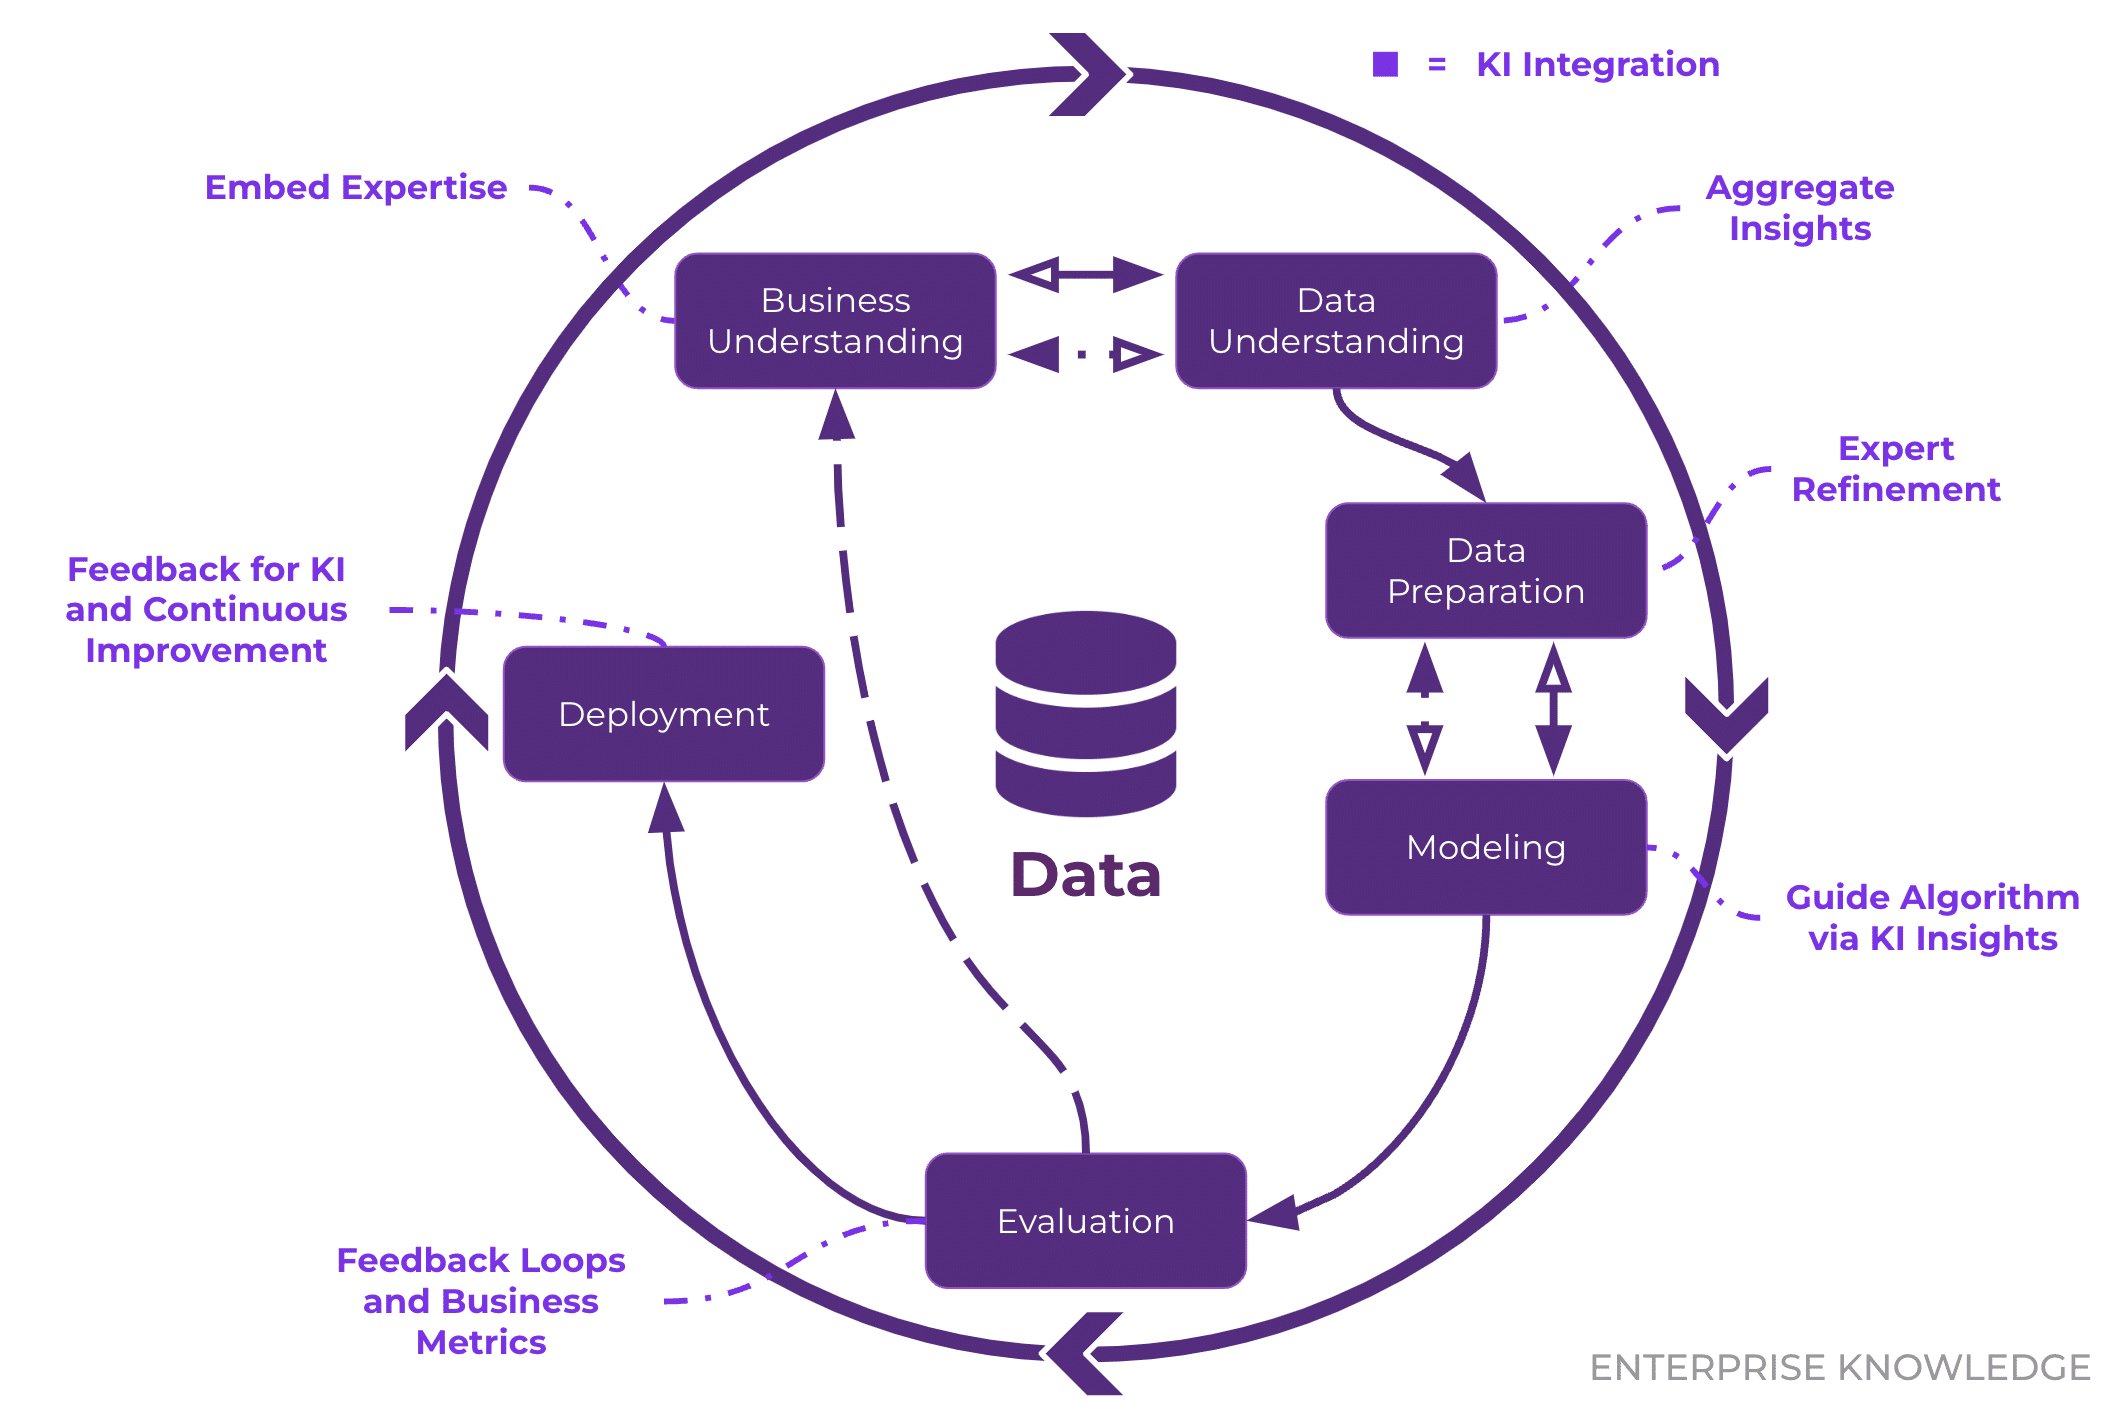
\includegraphics[width=0.8\textwidth]{figures/CRISP-DM.png}
\caption{CRISP-DM Methodology Phases \cite{chapman2000crispdm}}
\label{fig:crisp-dm}
\end{figure}

While \ac{CRISP-DM} has been widely adopted in traditional data mining and analytics 
projects, its linear progression and narrow focus on pattern extraction from existing 
datasets make it ill-suited for projects that involve designing and deploying an 
intelligent system from the ground up. It provides no framework for artifact 
construction, formal evaluation of system utility, or academic communication of 
results \cite{chapman2000crispdm}.

\subsection{Overview of TDSP}

\ac{TDSP} \cite{microsoft2016tdsp} is a more recent methodology developed specifically 
for \ac{AI} and machine learning projects in enterprise environments. First released 
in 2016, it combines agile principles with a structured data science lifecycle to 
address the challenges of building intelligent applications intended for production 
deployment.

The methodology is built on four core components \cite{microsoft2016tdsp}:

\begin{itemize}
    \item \textbf{Data Science Lifecycle:} An iterative process guiding projects from 
    business understanding through to deployment and continuous improvement.
    \item \textbf{Standardized Project Structure:} Consistent templates and folder 
    organization that promote team collaboration and reproducibility.
    \item \textbf{Infrastructure Recommendations:} Guidelines for cloud resources, 
    development environments, and deployment platforms.
    \item \textbf{Tool and Utility Guidance:} A curated selection of frameworks and 
    libraries supporting the entire \ac{AI} development pipeline.
\end{itemize}

\begin{figure}[H]
\centering
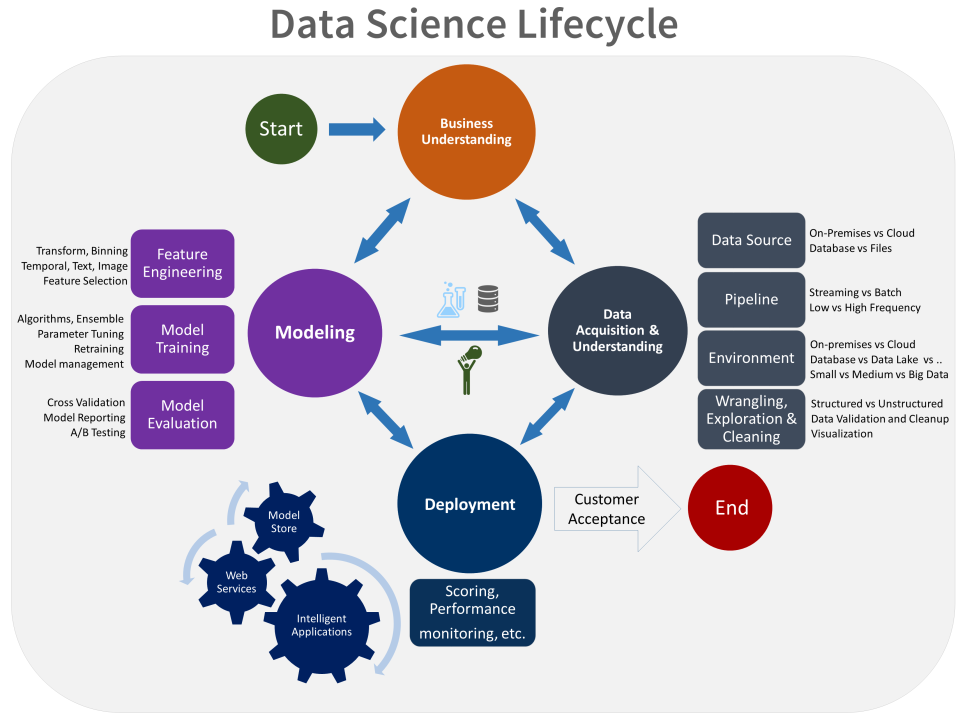
\includegraphics[width=0.8\textwidth]{figures/TDSP.png}
\caption{TDSP Iterative Lifecycle \cite{microsoft2016tdsp}}
\label{fig:tdsp-iterative}
\end{figure}

Although \ac{TDSP} represents a significant improvement over \ac{CRISP-DM} for 
modern \ac{AI} projects, it remains fundamentally an industry-oriented engineering 
framework. It does not provide a formal mechanism for artifact-centered research, 
rigorous academic evaluation, or scientific communication of results, all of which 
are essential requirements for an academic graduation project \cite{microsoft2016tdsp}.

\subsection{Overview of DSR}

\ac{DSR} \cite{hevner2004design, peffers2007dsrm} is a well-established research 
paradigm in information systems and computer science, specifically designed for 
projects whose primary output is a technological artifact, a system, model, method, 
or tool, built to solve a clearly identified real-world problem. Unlike traditional 
process methodologies, \ac{DSR} is rooted in a scientific approach: it requires not 
only that an artifact be constructed, but that its utility and effectiveness be 
formally evaluated and communicated as a research contribution 
\cite{hevner2004design}.

The \ac{DSR} process model \cite{peffers2007dsrm} consists of six iterative 
activities:

\begin{itemize}
    \item \textbf{Problem Identification and Motivation:} Defining the research 
    problem and justifying the value of developing a solution.
    \item \textbf{Definition of Objectives:} Specifying what a successful artifact 
    must achieve, derived directly from the problem definition.
    \item \textbf{Design and Development:} Constructing the artifact, encompassing 
    data collection, model training, system architecture, and integration.
    \item \textbf{Demonstration:} Deploying and using the artifact to solve the 
    identified problem in a realistic setting.
    \item \textbf{Evaluation:} Assessing how well the artifact addresses the problem 
    using appropriate metrics, comparisons, and validation techniques.
    \item \textbf{Communication:} Disseminating the problem, the artifact, and the 
    findings to relevant audiences through academic reporting and presentation.
\end{itemize}

\begin{figure}[H]
\centering
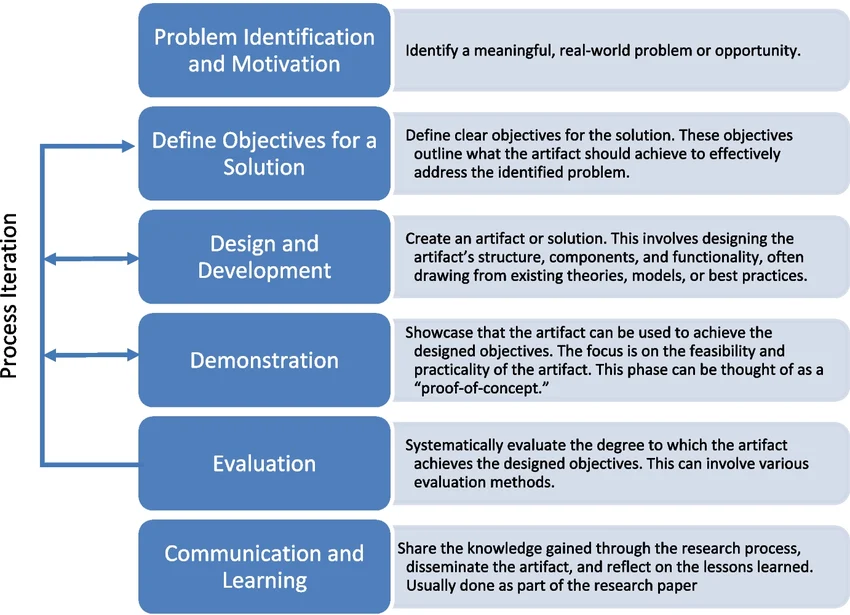
\includegraphics[width=0.9\textwidth]{figures/DSR.png}
\caption{DSR Process Model \cite{peffers2007dsrm}}
\label{fig:dsr}
\end{figure}

\subsection{Methodologies Comparison}

Table~\ref{tab:methodology-comparison} presents a structured comparison of the three 
methodologies across criteria relevant to the specific requirements of our project.

\begin{table}[H]
\centering
\caption{Comparative Analysis of CRISP-DM, TDSP, and DSR}
\label{tab:methodology-comparison}
\renewcommand{\arraystretch}{1.3}
\begin{tabular}{|p{3cm}|p{3.8cm}|p{3.8cm}|p{3.8cm}|}
\hline
\textbf{Criteria} & \textbf{CRISP-DM} & \textbf{TDSP} & \textbf{DSR} \\
\hline
Primary Focus & 
Data mining and pattern extraction & 
Production AI and ML systems & 
Design and evaluation of technological artifacts \\
\hline
Development Approach & 
Linear, sequential & 
Agile, iterative & 
Iterative, artifact-centered \\
\hline
Academic Rigor & 
Low & 
Low & 
High \\
\hline
Evaluation Framework & 
Basic model metrics & 
Deployment monitoring & 
Formal utility and efficacy assessment \\
\hline
Artifact Orientation & 
None & 
Partial & 
Central \\
\hline
Communication Phase & 
Not included & 
Not included & 
Explicitly included \\
\hline
Deployment Guidance & 
Basic system integration & 
Detailed production recommendations & 
Demonstration in realistic environment \\
\hline
Suitability for Small-Scale Projects &
Weak &
Moderate &
Strong \\
\hline
\end{tabular}
\end{table}

\subsection{Why We Chose DSR}

The comparative analysis reveals that \ac{DSR} \cite{hevner2004design, peffers2007dsrm} 
is the methodology best aligned with the nature and objectives of our project, for 
the following reasons:

\begin{itemize}
    \item \textbf{Artifact-Centered:} Our project's primary deliverable is a 
    specialized legal chatbot, a concrete technological artifact. \ac{DSR} is built 
    precisely around the design, construction, and evaluation of such artifacts 
    \cite{hevner2004design}.
    \item \textbf{Academic Rigor:} Unlike \ac{CRISP-DM} and \ac{TDSP}, \ac{DSR} 
    provides a formal evaluation framework that allows the utility and performance of 
    the system to be rigorously assessed, an essential requirement for an academic 
    graduation project.
    \item \textbf{Structured Evaluation:} The dedicated evaluation phase enables a 
    principled comparison between the fine-tuned model and a generic baseline, 
    providing scientifically grounded evidence of improvement \cite{peffers2007dsrm}.
    \item \textbf{Communication Phase:} Unlike \ac{CRISP-DM} and \ac{TDSP}, \ac{DSR}
    treats communication as a first-class activity rather than an afterthought, requiring
    researchers to document and disseminate the artifact, the design decisions, and the
    evaluation results to a relevant audience \cite{peffers2007dsrm}. This maps naturally
    onto the written report and oral defense that conclude this graduation project.
    \item \textbf{Iterative by Design:} The build-and-evaluate cycle at the core of 
    \ac{DSR} \cite{hevner2004design} naturally accommodates the multiple iterations 
    of fine-tuning, testing, and refinement that domain adaptation of a language model 
    requires.
\end{itemize}

\subsection{Our Adapted DSR Lifecycle}

We tailored the \ac{DSR} lifecycle \cite{peffers2007dsrm} to fit the specific 
structure of our project, embedding the full \ac{AI} technical pipeline within the 
Design and Development phase:

\textbf{Phase 1: Problem Identification and Motivation.}
We identified the core limitations of E-Tafakna's existing \ac{AI} agents, 
insufficient Tunisian legal knowledge and dependency on external cloud services, 
and established the need for a domain-specific, locally deployable solution.

\textbf{Phase 2: Definition of Objectives.}
We defined three concrete objectives for the artifact: domain adaptation through 
fine-tuning on Tunisian legal corpora, dynamic knowledge retrieval through a 
\ac{RAG} pipeline, and full on-premises deployment at \ac{ATI} Tunisie.

\textbf{Phase 3: Design and Development.}
This phase encompasses the complete \ac{AI} technical pipeline:
\begin{itemize}
    \item Collection and preprocessing of Tunisian legal documents.
    \item Fine-tuning of the base \ac{SLM} or \ac{LLM} on legal data.
    \item Design and implementation of the \ac{RAG} pipeline and vector database.
    \item Integration of the complete system into E-Tafakna's platform architecture.
\end{itemize}

\textbf{Phase 4: Demonstration.}
The artifact is deployed on \ac{ATI} Tunisie's on-premises infrastructure and 
demonstrated through realistic legal consultation scenarios covering the use cases 
of both Elyssa and Kahina.

\textbf{Phase 5: Evaluation.}
The system is evaluated using quantitative metrics (including response accuracy, 
legal precision, and retrieval quality) and compared against a generic baseline 
model to measure the concrete contribution of domain-specific fine-tuning.

\textbf{Phase 6: Communication.}
The findings, artifact design, and evaluation results are communicated through this 
academic report and its oral defense before the graduation jury.

\section{Choice of Services, Technologies, and Tools}
\label{sec:tools-choice}

Beyond selecting a methodological framework, the successful execution of our project 
required identifying the right set of services and technologies to support its different 
phases. This section presents the main platform we relied on during the design and 
development of our solution, and explains the rationale behind its selection.

\subsection{Azure AI Foundry: Access to State-of-the-Art Language Models}

Azure AI Foundry is Microsoft's unified platform for building, evaluating, and deploying 
generative \ac{AI} applications. It provides centralized access to a catalog of foundation 
models from multiple providers (including OpenAI, Meta, and Mistral) through a single 
secure endpoint, along with tooling for prompt engineering, model evaluation, and 
enterprise-grade governance \cite{microsoft2024azureaifoundry}.

\begin{figure}[H]
\centering

\includegraphics[width=0.4\textwidth]{figures/azure_ai_foundry.jpg}
\caption{Azure AI Foundry Platform \cite{microsoft2024azureaifoundry}}
\label{fig:azure-ai-foundry}
\end{figure}

Within this ecosystem, we specifically relied on the \textbf{GPT-4.1} model made available 
through Azure OpenAI Service. GPT-4.1 is one of the most advanced large language models 
offered on the platform, featuring an expanded context window, strong multimodal 
capabilities, and improved instruction following compared to previous generations, 
characteristics that are particularly valuable when processing dense and heterogeneous 
legal documents \cite{microsoft2024azureopenai}.

\subsubsection*{Role in Our Project}

GPT-4.1 played a central role in the data preparation phase of our project. The Tunisian 
legal corpus required for fine-tuning was originally available as a large collection of 
PDF documents (including legislation, official gazettes, and regulatory texts) whose 
content was often embedded in complex layouts, multi-column formats, and scanned pages. 
Traditional text extraction tools proved insufficient to reliably capture the structure 
and semantics of these documents.

To overcome this limitation, we used GPT-4.1 as an intelligent extraction engine capable 
of:

\begin{itemize}
    \item \textbf{Accurate Text Extraction:} Converting raw PDF content into clean, 
    structured text while preserving the hierarchical organization of legal documents 
    (articles, sections, and clauses).
    
    \item \textbf{Semantic Structuring:} Identifying and labeling key components of legal 
    texts, such as article numbers, titles, and references to other legal provisions.
    
    \item \textbf{Noise Removal:} Filtering out irrelevant artifacts introduced by the 
    PDF format, including headers, footers, page numbers, and watermarks.
\end{itemize}

The output of this extraction process served as the foundation of our curated Tunisian 
legal dataset, which was subsequently used for fine-tuning the target language model and 
populating the vector database of the \ac{RAG} pipeline.

\subsubsection*{Rationale for Selection}

{\itshape Azure AI Foundry was chosen for its enterprise-grade security guarantees, its native 
integration with other Azure services, and its compliance with data protection standards, 
all of which align with the confidentiality requirements of legal data handling. 
Although the final production system is deployed entirely on-premises at \ac{ATI} 
Tunisie, leveraging GPT-4.1 during the data preparation phase allowed us to build a 
high-quality legal corpus efficiently, without compromising the on-premises nature of 
the final deliverable.}

\subsection{Google Vertex AI: OCR Extraction from Image-Based PDFs}

Google Vertex AI is Google Cloud's unified machine learning platform, bringing together
a broad suite of \ac{AI} services (including foundation models, AutoML, custom training,
and managed inference) under a single \ac{API} and console \cite{google2024vertexai}.
Among its services, \textbf{Document AI} provides enterprise-grade document processing
capabilities, including optical character recognition (\ac{OCR}), form parsing, and
intelligent document splitting \cite{google2024documentai}.

\begin{figure}[H]
\centering

\includegraphics[width=0.4\textwidth]{figures/vertex_ai_logo.png}
\caption{Google Vertex AI \cite{google2024vertexai}}
\label{fig:vertex-ai-logo}
\end{figure}

\subsubsection*{Role in Our Project}

A significant portion of the Tunisian legal corpus was available only as scanned
image-based \ac{PDF} files, meaning the content was stored as rasterized images
rather than selectable text, making standard text extraction tools entirely
ineffective. To handle this category of documents, we relied on Google Vertex AI's
Document AI \ac{OCR} capabilities, which can process image-based \ac{PDF} pages and
return high-accuracy text output by performing character recognition directly on the
visual content.

Specifically, Vertex AI Document AI was used to:

\begin{itemize}
    \item \textbf{Optical Character Recognition (OCR) Processing:} Extract machine-readable text from scanned legal
    documents where the content existed solely as images, covering legislation texts,
    official gazettes, and regulatory decrees unavailable in digital form.

    \item \textbf{Multi-page Document Handling:} Process lengthy \ac{PDF} files
    spanning hundreds of pages in batch, returning structured text output that could
    be integrated into the same data pipeline as digitally-born documents.

    \item \textbf{Arabic and French Script Recognition:} Accurately recognize both
    Arabic and French characters present in Tunisian legal texts, given that many
    official documents are bilingual.
\end{itemize}

The extracted text was then passed through the same cleaning and structuring pipeline
used for the digitally-born documents, ensuring a uniform representation across the
entire legal corpus.

\subsubsection*{Rationale for Selection}

{\itshape Google Vertex AI Document AI was selected specifically for its strong multilingual
\ac{OCR} performance on Arabic-script and Latin-script documents, a critical
requirement given the bilingual nature of the Tunisian legal corpus. Its cloud-based
batch processing model also allowed us to handle large volumes of scanned documents
without requiring local infrastructure during the data preparation phase, while the
final production system remained fully on-premises at \ac{ATI} Tunisie.}

\subsection{OVH AI Notebooks: GPU Resources for Fine-Tuning}

OVH AI Notebooks is a managed cloud service provided by OVHcloud that delivers
on-demand Jupyter notebook environments backed by dedicated \ac{GPU} instances.
It is designed to make computationally intensive \ac{AI} workloads accessible
without the overhead of provisioning and maintaining dedicated hardware, giving
practitioners direct access to \ac{GPU} resources through a familiar notebook
interface \cite{ovh2024notebooks}.

\begin{figure}[H]
\centering

\includegraphics[width=0.35\textwidth]{figures/ovh_logo.png}
\caption{OVHcloud AI Notebooks \cite{ovh2024notebooks}}
\label{fig:ovh-notebooks}
\end{figure}

\subsubsection*{Role in Our Project}

Fine-tuning a large language model on a domain-specific corpus is among the most
computationally demanding tasks in the \ac{AI} pipeline. Running such a workload
on a standard development machine would require days or even weeks of processing
time, making rapid experimentation practically impossible. To address this, we
used OVH AI Notebooks to run the fine-tuning experiments on \ac{GPU}-accelerated
instances, which dramatically reduced training time and allowed us to iterate
efficiently over different configurations:

\begin{itemize}
    \item \textbf{Fine-Tuning Execution:} Running the supervised fine-tuning
    pipeline on the curated Tunisian legal corpus, leveraging \ac{GPU} acceleration
    to complete training jobs in a fraction of the time that would be required on
    standard hardware.

    \item \textbf{Experiment Tracking:} Using the notebook environment to monitor
    training metrics, compare runs, and adjust hyperparameters interactively between
    iterations.

    \item \textbf{Model Evaluation:} Running inference on the fine-tuned checkpoints
    directly within the notebook environment to perform initial quality assessments
    before moving to formal evaluation.
\end{itemize}

\subsubsection*{Rationale for Selection}

{\itshape OVH AI Notebooks was chosen for the combination of accessible \ac{GPU} capacity,
competitive pricing, and European data residency, a relevant consideration given the
legal sensitivity of the training data. Its notebook-native interface integrated
smoothly with our existing Python and Hugging Face Transformers workflow, avoiding
the need to learn a new toolchain. As with the other cloud services used during
data preparation, the reliance on OVH was limited strictly to the training phase.
The final production system remains entirely self-contained and deployed on-premises
at \ac{ATI} Tunisie.}

\subsection{Visual Studio Code}

Visual Studio Code is a free, lightweight code editor maintained by Microsoft. 
While it remains light on system resources, it can be extended to support 
virtually any language or workflow through its extension marketplace, and 
brings together editing, debugging, version control, and a built-in terminal 
within a single interface \cite{microsoft2024vscode}.

\begin{figure}[H]
\centering

\includegraphics[width=0.15\textwidth]{figures/vscode_logo.png}
\caption{Visual Studio Code \cite{microsoft2024vscode}}
\label{fig:vscode-logo}
\end{figure}

\subsubsection*{Role in Our Project}

VS Code acted as the single workspace where most of the technical work took 
place. Its versatility allowed us to handle several aspects of development 
without leaving the editor:

\begin{itemize}
    \item \textbf{Python Development:} Writing and debugging the data 
    preparation routines, the fine-tuning scripts, and the \ac{RAG} integration 
    code, with the help of the official Python extension and interactive 
    Jupyter notebooks.
    
    \item \textbf{Version Control:} Managing the project's source code directly 
    through the built-in Git interface, which made tracking changes and 
    navigating the project history straightforward.
    
    \item \textbf{Integrated Terminal:} Launching training jobs, installing 
    dependencies, and running command-line utilities from within the editor 
    itself, avoiding the need to jump between different windows.
\end{itemize}

\subsubsection*{Rationale for Selection}

{\itshape We chose VS Code mainly for practical reasons: it runs smoothly on modest 
hardware, supports the full Python ecosystem we needed, and brings editing, 
debugging, and version control together in one interface. Keeping everything 
in a single workspace noticeably reduced the friction of switching between 
tasks, which matters in a project that combines data handling, model training, 
and integration work.}

\subsection{Python}

Python is a high-level, interpreted programming language known for its clear 
syntax and the maturity of its scientific and \ac{AI} libraries. It is today 
the most widely adopted language in the \ac{AI} and machine learning community, 
largely because of the richness of its ecosystem around data processing, model 
training, and evaluation \cite{python2024docs}.

\begin{figure}[H]
\centering

\includegraphics[width=0.15\textwidth]{figures/python_logo.png}
\caption{Python Programming Language \cite{python2024docs}}
\label{fig:python-logo}
\end{figure}

\subsubsection*{Role in Our Project}

Python served as the main language for every technical component of our 
solution. Its rich ecosystem allowed us to cover the entire \ac{AI} pipeline 
without having to mix multiple languages:

\begin{itemize}
    \item \textbf{Data Processing:} Cleaning and restructuring the Tunisian 
    legal corpus extracted from \ac{PDF} documents, using libraries such as 
    Pandas and NumPy.
    
    \item \textbf{Model Fine-Tuning:} Building the fine-tuning pipeline around 
    widely used \ac{AI} frameworks, including Hugging Face Transformers and 
    PyTorch.
    
    \item \textbf{RAG Pipeline Development:} Implementing the different stages 
    of the retrieval-augmented generation workflow, from embedding generation 
    to vector store queries and orchestration of the overall flow.
    
    \item \textbf{Scripting and Automation:} Writing smaller utility scripts 
    to automate recurring tasks such as dataset preparation, evaluation runs, 
    and aggregation of results.
\end{itemize}

\subsubsection*{Rationale for Selection}

{\itshape Python was chosen for its central role in the \ac{AI} ecosystem and the 
availability of mature libraries covering every stage of our pipeline, from 
data extraction to model training, evaluation, and deployment. Its readability 
also made the codebase easier to document and maintain, which was particularly 
valuable in the academic context of this project.}

\subsection{n8n}

n8n is an open-source workflow automation platform that allows users to design 
processing pipelines visually, by connecting nodes that each perform a specific 
action, from calling an \ac{API} to reading a file or running a script. It 
can be fully self-hosted, meaning workflow data never has to leave the local 
environment \cite{n8n2024docs}.

\begin{figure}[H]
\centering

\includegraphics[width=0.3\textwidth]{figures/n8n_logo.png}
\caption{n8n Workflow Automation Platform \cite{n8n2024docs}}
\label{fig:n8n-logo}
\end{figure}

\subsubsection*{Role in Our Project}

n8n was used to orchestrate the different stages of our processing pipeline. 
Rather than chaining scripts manually or writing a dedicated runner, we built 
workflows that trigger each step in the right order and give us a clear visual 
overview of the whole process:

\begin{itemize}
    \item \textbf{Data Pipeline Orchestration:} Coordinating the sequence of 
    operations involved in preparing the legal corpus, from raw document 
    ingestion to structured output generation.
    
    \item \textbf{API Integration:} Connecting the different components of 
    the system through \ac{HTTP} calls, which simplified communication between 
    services without adding custom glue code.
    
    \item \textbf{Process Automation:} Scheduling and triggering recurring 
    tasks automatically, reducing manual work and keeping pipeline executions 
    consistent.
\end{itemize}

\subsubsection*{Rationale for Selection}

{\itshape n8n was selected mainly because it is open-source and self-hostable, which 
aligns with the on-premises deployment constraints imposed by \ac{ATI} Tunisie. 
Beyond that, its visual approach lowered the overhead of managing a growing 
number of processing steps, and the ability to keep everything on local 
infrastructure ensured that no data ever left the controlled environment 
during automated processing.}

\subsection{FastAPI}

FastAPI is a modern Python web framework used to expose code as \ac{HTTP} 
services. It is designed around Python type hints, which it leverages to 
validate requests automatically and generate interactive documentation, while 
offering strong performance thanks to its native support for asynchronous 
operations \cite{fastapi2024docs}.

\begin{figure}[H]
\centering

\includegraphics[width=0.25\textwidth]{figures/fastapi_logo.png}
\caption{FastAPI Framework \cite{fastapi2024docs}}
\label{fig:fastapi-logo}
\end{figure}

\subsubsection*{Role in Our Project}

FastAPI served as the bridge between our Python scripts and the n8n automation 
platform. Since n8n interacts with external services through \ac{HTTP} calls, 
we wrapped our extraction and \ac{RAG}-related scripts behind small FastAPI 
endpoints so that n8n workflows could invoke them like any other integration:

\begin{itemize}
    \item \textbf{Script Exposition:} Turning standalone Python scripts, 
    including the legal data extraction routines and the \ac{RAG} pipeline 
    components, into \ac{HTTP} endpoints that could be consumed directly from 
    n8n.
    
    \item \textbf{Seamless Orchestration:} Allowing n8n to trigger Python 
    operations as part of larger automated workflows, keeping a clean 
    separation between orchestration on one side and execution on the other.
    
    \item \textbf{Automatic Validation and Documentation:} Relying on FastAPI's 
    type-based validation and auto-generated interactive interface to speed up 
    the development and testing of each endpoint.
\end{itemize}

\subsubsection*{Rationale for Selection}

{\itshape FastAPI was chosen because it makes exposing Python functions as web endpoints 
almost trivial, while still offering solid performance under the kind of 
long-running inference calls our pipeline involves. Its native support for 
asynchronous operations fit naturally with our \ac{AI} workloads, and its 
tight integration with the Python ecosystem made it the most practical choice 
to connect our processing scripts to the n8n automation layer.}

\section{Conclusion}

This chapter introduced E-Tafakna and its existing \ac{AI} agents, identified the
two core limitations of the current system, namely the lack of Tunisian legal
grounding and the dependency on external cloud services, and proposed a solution
combining a fine-tuned language model, a \ac{RAG} pipeline, and fully on-premises
deployment at \ac{ATI} Tunisie. We also selected \ac{DSR} as our guiding methodology,
given its artifact-centered structure and formal evaluation framework.

The following chapter grounds this project in the existing literature, examining
the key concepts and technologies that underpin our proposed solution.